	%====================================================================================================
	% ?????
	%====================================================================================================
	% TCC
	%----------------------------------------------------------------------------------------------------
	% Autor				: Jasane Schio
	% Orientador		: Gedson Faria
	% Co-Orientador		: Angelo Darcy
	% Instituição 		: UFMS - Universidade Federal do Mato Grosso do Sul
	% Departamento		: CPCX - Sistema de Informação
	%----------------------------------------------------------------------------------------------------
	% Data de criação	: 01 de Outubro de 2015
	%====================================================================================================
	%descrever problemas e as solucoes encontradas
	\definecolor{dkgreen}{rgb}{0,0.6,0}
	\definecolor{gray}{rgb}{0.5,0.5,0.5}
	\definecolor{mauve}{rgb}{0.58,0,0.82}
	
	\lstset{frame=tb,
		language=C++,
		aboveskip=3mm,
		belowskip=3mm,
		showstringspaces=false,
		columns=flexible,
		basicstyle={\small\ttfamily},
		numbers=none,
		numberstyle=\tiny\color{gray},
		keywordstyle=\color{blue},
		commentstyle=\color{dkgreen},
		stringstyle=\color{mauve},
		breaklines=true,
		breakatwhitespace=true,
		tabsize=3
	}
	\chapter{Desenvolvimento} 
	
			Para o desenvolvimento foi escolhida a biblioteca OpenCV por ser OpenSource, multiplataforma, conter uma grande quantidade de métodos e algoritmos já implementados	e pelo seu rápido desempenho de máquina.
			A linguagem escolhida para o desenvolvimento foi o C++ pois é uma linguagem de programação compilada, o que torna sua execução mais rápida que as linguagem interpretadas, dando ao sistema grande 
\section{Tecnologias Usadas}
Para realização deste trabalho, irei utilizar a biblioteca de processamentos de imagens conhecida como OpenCV: Open Source Computer Vision Library. O trabalho será elaborado na linguagem C++, com uso do framework Qt para sua interface gráfica.
Os passos detalhados do projeto e seu desenvolvimento estará presente no Capítulo de Metodologia.
\begin{description}
	\item[OpenCV] Lançado em 1999 pela Intel\cite{Culjak:2012}, com objetivo de ser otimizada, portável e com um grande número de funções, o Open Source Computer Vision Library,OpenCV, se tornou se tornou uma ferramenta que possui mais de 2500 algoritmos e 40 mil pessoas em seu grupo de usuários\cite{Culjak:2012}. Já possui interface para as linguagens C++, C, Python e Java além de suporte para as principais plataformas com Windows, Linux, Mac OS, iOS e Android. A biblioteca lida tanto com imagens em tempo real, como vídeos e imagens estáticas.
	
	\item[Qt] Qt é um framework de desenvolvimento de aplicações multiplataforma. Entre suas funcionalidades está a possibilidade de criar interfaces gráficas diretamente em C ++ usando seu módulo Widgets.
	
	\item [C++] A linguagem de programação C++ foi projetado por Bjarne Stroustrup para fornecer eficiência e flexibilidade da linguagem C para programação de sistemas. A linguagem evoluiu a partir de uma versão anterior chamado C com Classes, o projeto C com Classes durou entre 1979 e 1983 e determinou os moldes para o C++. A linguagem foi oficialmente lancada em 1986.\cite{Stroustrup:1996} 
\end{description}

\section{Projeto}
\subsection{Organização do Projeto}
	 O projeto foi desenvolvido seguindo o paradigma de programação Orientada à Objetos, esse paradigma baseia-se na utilização de objetos individuais para criação de um sistema maior e complexo. A IDE usada para o desenvolvimento foi a QT Creator, esta separada o projeto em três pastas, Headers, Sources e Forms. Na pasta Headers estão os arquivos de cabeçalho(.h) onde estão as declarações dos métodos e variáveis usados nas classes  executáveis. Já na pasta Sources estão os arquivos fonte(.cpp), são nesses arquivos que os métodos declarados nos arquivos da pasta Header são implementados. Na pasta Forms está o arquivo de interface gráfica(.ui) que é usado no projeto para ser a ponte entre o usuario e as funções do sistema.
	 
	\begin{figure}[!h]
		\centering
		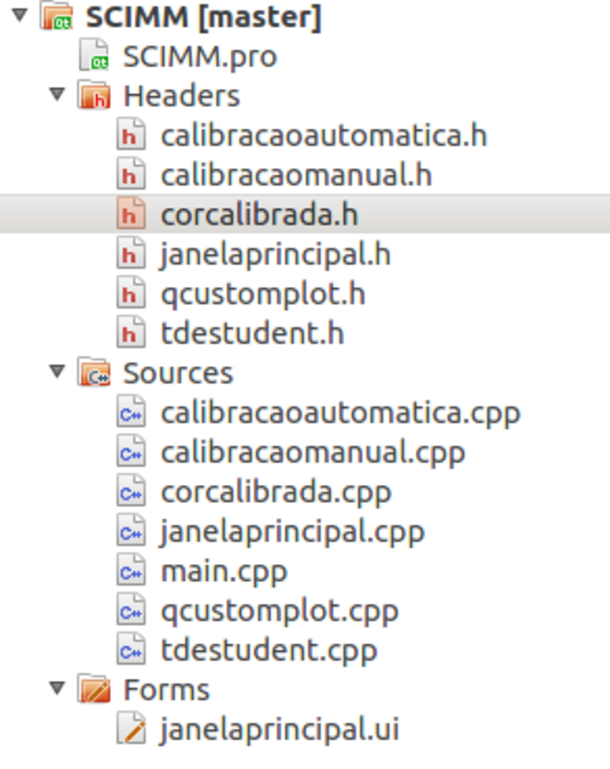
\includegraphics[width=0.2\textwidth]{organizacaoProjeto.pdf}
		\caption{Organização das pastas do projeto}
		\label{Organizacao do Projeto}
	\end{figure}
	Cada arquivo de cabeçalho possui um arquivo fonte correspondente, formando assim uma Classe, com exceção do arquivo fonte main, pois para este arquivo não há a necessidade.
	As classes desenvolvidas no projeto são: calibracao, automatica, scimm\_cor, janelaprincipal.
%Para melhor entendimento da interação entre as classes a figura 3.2 trás o diagrama de classes do projeto.

\subsection{Classes}
\subsubsection{main}
 Esta é o que se chama de \textit{ponto de entrada} em programação.\textit{Ponto de entrada} é onde o sistema operacional ira iniciar a execução do sistema desenvolvido. Esta classe possui somente o metodo \textbf{main} e este invoca a classe \textbf{JanelaPrincipal} que apresenta a interfaçe grafica para interação com o usuario, e de acordo com esta interação iniciar o processo de calibração.
 
\subsubsection{JanelaPrincipal}
É uma classe-objeto que utiliza da implementação de objetos QWidget e suas subclasses disponiveis pelo framework Qt, para a criação de uma interface grafica que faz a interação com o usuario e que seleciona o tipo de calibração a ser iniciada. Todos os metodos presentes nessa clase são para utilização grafica, ex. comportamento de botões, slider, abas, menus de seleção, gráficos, bem como a comunicação com as classes de calibração.	

\subsubsection{Calibracao}
 É classe que contem os metodos e variaveis proprios além dos oriundos da classe base \textbf{Calibracao} e os implementa de acordo com a necessidade da calibração manual:
 
Os métodos da propria classe são:
	\begin{description}

\item Iniciar: Método onde é o ID da camera é fixado dentro da classe, também é o método que faz a gerencia dos metodos inciais. Incovando primeiro o metodo de configuração de imagem, durante o método \textbf{ConfigurarCamera} para se configurar a imagem, que sera analizada durante a calibração, onde é feita a tentativa de acesso a camera. Caso esta esteja disponivel a configuração finaliza e somente após a mesma finalizada se inicia a rotina de calibração, caso a camera esteja indiponivel a calibração fica impedida de iniciar.
	


\item ConfigurarCamera: Método onde a imagem de exibição é ajustando utilizando configurações de brilho, contraste e tamanho de tela.	
	
  \item ReconhecerFundo: Método que utiliza o algoritmo de subtração de fundo por mistura gaussiana para identificar o campo e fazer, mais tarde no método \textbf{ExtrairObjetos}, a detecção dos objetos que não fazem parte do campo para assim detectar os objetos com mais precisão, uma vez que os objetos-cor eram os unicos que não fazim parte da imagem inicial, o fundo.
  
	        \item ExtrairObjetos
 
	\item Calibrar: Método onde é exibido a imagem da camera e quando estiver de acordo com a exigencia do usuario o mesmo inicial a calibração. So apos ser iniciada a calibração o método \textbf{DetectarObjetos} é invocado, apos os objetos de cores serem identificados, é retornada à tela do usuario a lista do objetos.			
		
	\item DetectarObjetos: Método onde serão aplicados filtros de diminuição de ruido, detectadas as bordas existentes na imagem, detectados os objetos a partis das bordas contidas na imagem, o aumento da precisão dos objetos e diminuição do tamanho do objeto de acordo com a porcentagem de borda a ser eliminada. 

	\item ObterPorcentagem: Método simples para devolver a porcentagem de um valor, ao ser informado o valor  e a porcentagem escolhida.
		
		
		\item Calcular: Método onde cada pixel pertencente à cada um dos objetos encontrados é analisado e seus valores HSV adicionados a lista de ocorrencia. 
		O algoritmo de contagem de ocorrencia em cada pixel é dado da seguinte maneira:
 
	        
	        \begin{algorithm}
	       		 \caption{Contagem dos Valores HSV}
		        \begin{algorithmic}
		     	
		     	\ForAll{objeto encontrado} 
		     		\ForAll{pixel do objeto} 
		   				 \State OcorrenciasDeH[pixel.h]++ 
		    			 \State	OcorrenciasDeS[pixel.s]++ 
		     	  		 \State	OcorrenciasDeV[pixel.v]++
		     	   \EndFor
		     	\EndFor
		     		
		        \end{algorithmic}
	        
	        \end{algorithm}
	        
	        
	        
	        
	      
		\end{description}	

\subsubsection{SCIMM\_COR}



\section{O Sistema}

		\begin{figure}[!h]
			\centering
			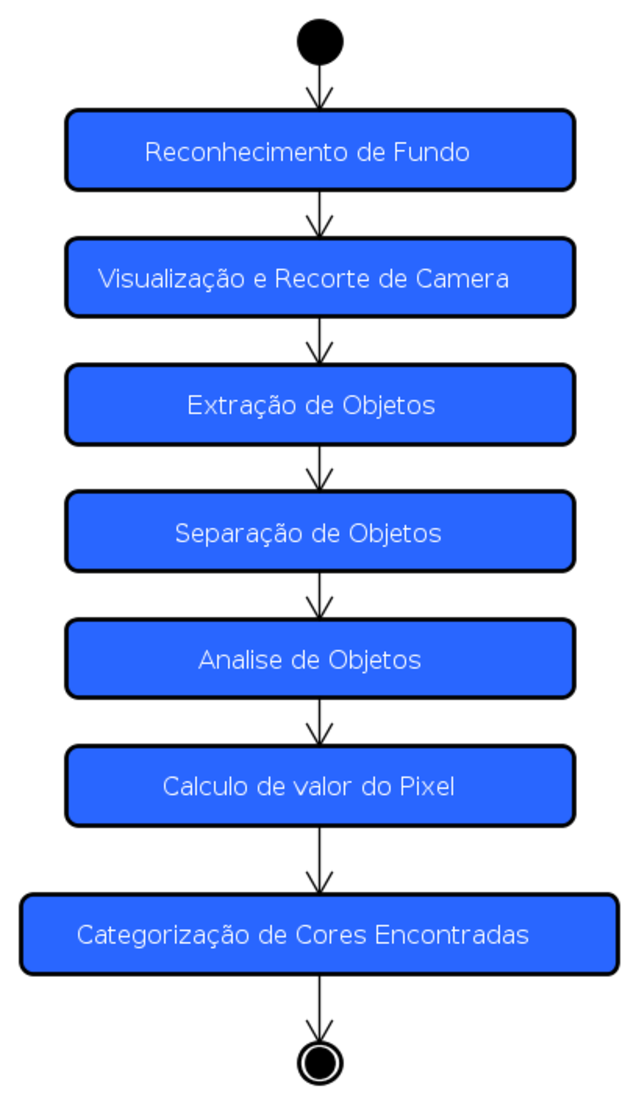
\includegraphics[width=0.45\textwidth]{FluxodoSistema.pdf}
			\caption{Diagrama de Fluxo}
			\label{FlowCHart}
		\end{figure}
		A Figura 3.3 mostra o diagrama de fluxo do sistema de calibraçao.
		
		 O sistema consiste na apresentação da \textbf{interface gráfica} ao usuario. A \textbf{interface grafica} que por sua vez oferece as duas possibilidades ao usuario, de acordo com o tipo de calibração escolhido o sistema inicia a rotina de calibração referente. Apos a execução de toda o sistema é finalizada.
			
	 
		Conformo mostrado na Figura \ref{DiagramaDeFluxoAutomatico} a rotina de calibração automatica possui cinco etapas. Este tipo de calibração  possui o mínimo possivel de interação com o usuario. O sistema faz automaticamente a detecção de objetos e utilizando a probabilidade matematica T de Student, considerando o tamanho de todos os objetos encontrados para encontrar os tamanhos minimo e maximo que os objetos desejados devem ter, nesse caso as etiquetas de cores dos robos, e só após determinar quais objetos possuem o tamanho desejado, analisar os valores e calcular as ocorrencias de cada um dos três valores do modelo HSV.
			Nas subsessões à seguir explicarei detalhadamente cada uma das etapas do processo de calibração automatica
	

	\subsection{1ª Etapa - Reconhecimento de Fundo}
	Um principais problemas que ocorrem na detecçao de objetos é a confusão do fundo junto ao proprio objeto, fazendo assim que o mesmo seja detectado porem nao seu contorno correto, ou em outras vezes ignorado por ser considerado parte do fundo. Para eliminar este problema foi utilizado a tecnica  Subtração do fundo usando Mistura de Gaussianas, por meio do objeto \textit{createBackgroundSubtractorMOG2()} disponivel na biblioteca \textit{OpenCV}. Esta tecnica utiliza um algoritmo de analise pixel a pixel e que classifica o mesmo baseando-se na distribuição da gaussiana que o representa. Para separar o fundo do resto da imagem é levada em consideração que a gaussiana que representa o fundo tenha grande pesso e baixa variância, isso significa que a mesma ocorre frequentemente e varie pouco no tempo. O algoritmo atualiza o modelo de fundo a cada quadro da imagem baseando-se na variancia do objetos da mesma e de sua variancia. O objeto criado pela biblioteca, por meio do metodo \textbf{apply}, analisa quadro a quadro a imagem, a compara com o fundo obtido e gera uma imagem chamada de \textbf{mascara} com os objetos que nao fazem parte do fundo, no exato momento da imagem, com o passar dos quadros o objeto se torna parte do fundo. Uso do metodo:
\begin{center}
\centering \textit{pMOG2->apply(frame, fgMaskMOG2);}
\end{center}

Onde \textbf{frame} significa a imagem atual capturada pela camera e \textbf{fgMaskMOG2} a mascara gerada pela diferença da imagem atual com o modelo de fundo. 

Sabendo inicialmente que o modelo de fundo do objeto \textbf{pMOG2} esta vazio, basta que ele seja executado algumas vezes para que o campo se torne o modelo de fundo. Nesse caso a mascara gerada pelo metodo não chega a ser utilizada, porem sera na 3ª etapa.
	\subsection{2ª Etapa - Configuração de Camera}
		

Para melhor desempenho do algoritmo de detecçao de objetos, a imagem é recortada somente para o tamanho necessario do campo. O recorte de imagem foi feito utilizando a função setMouseCallback para possibilitar a interção do usuario na imagem por meio do mouse, sua utilização é dada da seguinte maneira:
\begin{center}
\centering \textit{ cv::setMouseCallback(src\_window,mouseHandler,0);}
\end{center}
Tem como primeiro parametro \textbf{src\_windows} que indica a janela na qual a função recebera a interação,  o segundo, \textbf{mouseHandler}, indica a função na qual esta implementada a interação e o ultimo parametro, \textbf{0}, indica parametros opcionais, neste caso não usaremos nenhum então foi usado o numero 0.
Dentro da função \textbf{mouseHandler} são identificados os pontos iniciai e final da seleção na tela e utilizada a função \textit{rectangle} para demarcar a seleção na tela. A utilização da função \textit{rectangle} completa fica da seguinte maneira:
\begin{center}
\centering \textit{ cv::rectangle(frameA, point1, point2, CV\_RGB(255, 0, 0), 2, 5, 0);}
\end{center}
A função rebece os parametros \textbf{frameA} indicando a imagem na qual será demarcada a area selecionada, depois o parametro \textbf{point1} que é o ponto incial de seleção na imagem, \textbf{point2} que é o ponto final da seleção. \textbf{CV\_RGB(255, 0, 0)} que indica a cor da demarcação, \textbf{2} indicando a expessura da demarcação, \textbf{5} que significa o tipo de linha a ser utilizado na demarcação e \textbf{0} que é o numero de bits fracinarios.
 Após confirmada a escolha do tamanho da tela 
este é então salvo na variavel nomeada \textit{tamanho}, está então sera usado durante todo o processo de calibração.
	\subsection{3ª Etapa - Extração dos Objetos do Fundo}
	Como visto na 1ª etapa, o objeto \textbf{pMOG2} chamando o metodo \textit{apply} o mesmo gera uma mascara de diferença da imagem atual para o modelo de fundo. Sendo assim para obtermos os objetos que virao a ser detectados basta que o metodo \textit{apply} seja chamado um numero de vezes suficiente para criar a mascara e o mesmo nao alterar o modelo de fundo.
	
\subsection{4ª Etapa - Detecção e validação de Objetos}
A detecção dos objetos a serem calibrados é dada pelo algoritmo de detecção de bordas de Canny. Como mais um recurso para eliminação de ruidos e melhoria da imagem antes de ser executado a detecção de objetos atravez da detecção de bordas é utilizado desfoque na imagem. O algoritmo de Canny já está implementado dentro da biblioteca OpenCV e com a seguite usagem:
\begin{center}
\centering \textit{  Canny(src\_gray, canny\_output, limiar, limiar * 3, 3);}
\end{center}
O algoritmo de Canny utiliza por padrão imagem em padrões de cinza, sendo assim \textbf{src\_gray} é a imagem orignal tranformada para escala de cinza, esta é a imagem na qual o algoritmo sera aplicado. \textbf{canny\_output} será a imagem de saida da função.
\textbf{limiar} e \textbf{limiar*3} são os limites mínimos e máximos para considerar uma borda. \textbf{3} é o valor de apertura ou kernel, o valor 3 é utilizado como padro.

Apos o uso do algoritmo de Canny para detecção de bordas é necessario então fazer uso da função \textit{findContours}, nativa no \textit{OpenCV} para detecção de contornos.
\begin{center}
\centering \textit{ findContours(canny\_output, contours, hierarchy, CV\_RETR\_EXTERNAL, CV\_CHAIN\_APPROX\_SIMPLE, Point(0, 0))}
\end{center}

O primeiro parametro, \textbf{canny\_output}, é a imagem que o algoritmo de Canny gerou com as bordas encontrada na imagem, e é a imagem que o método \textit{findContours} ira utilizar para detectar os contornos, \textbf{contours} é o parametro que indica onde serão salvos os contornos encontrados, cada contorno é armazenado como sendo um vetor de pontos \cite{OpenCV}. \textbf{hierarchy} é onde será salva um verot de informações sobre a topologia da imagem, e terá como total de elementos o mesmo numero que o total de contornos encontrado\cite{OpenCV}. O quarto parametro, \textbf{CV\_RETR\_EXTERNAL} indica o modo de obtenção de contornos, nesse caso \textit{CV\_RETR\_EXTERNAL} indica que o metodo só obtera os contornos exteriores\cite{OpenCV}. \textbf{CV\_CHAIN\_APPROX\_SIMPLE} indica o metodo que sera usado para aproximação de contornos, o metodo \textit{CV\_CHAIN\_APPROX\_SIMPLE} comprime segmentos horizontais, verticais, diagonais e deixa apenas os seus pontos finais\cite{OpenCV}. E o ultimo parametro, \textbf{Point(0, 0)}, indica o valor a ser usado para deslocar a imagem ao encontrar os objetos, neste caso esse valor é 0 para Y e 0 para X, pois não sera necessario. 

Uma vez obtidos os contornos é necessarios que se faça a eliminação de vertices dos polignos encontrados nos objetos deixando assim o objeto mais preciso. Isso é necessario para deixar a forma encontrada mais precisa dá forma original. Para este ajuste foi usado o metodo \textit{approxPolyDP}, ja implementado dentro da biblioteca OpenCV. Esse metodo teve que ser aplicado em cada um dos contornos encontrados, e foi utilizado da seguinte maneira:
\begin{center}
\centering \textit{    approxPolyDP(Mat(contours[i]), contours\_poly[i], 3, true)}
\end{center}
 Onde o metodo inicia recebendo como paralametro, \textbf{Mat(contours[i])} que é a criação de uma nova imagem, somente com aquele unico objeto, que esta sendo analisado. A seguir é informado no segundo parametro a variavel de destino \textbf{contours\_poly[i]}, onde sera salvo o objeto com a eliminação dos vertices. O terceiro parametro indica o valor do \textit{epilson}, usado o valor \textbf{3} que especifica a precisão da aproximação, a distância máxima entre a curva original e a sua aproximação\cite{OpenCV}. O ultimo parametro indica se a curva aproximada sera fechada ou não, foi usado o valor \textbf{true} pois neste caso fechar um uma curva é necessario para que o objeto onde está a cor, seja idenficado e analisado na probabilidade.
 Por ultimo os objetos possuem sua borda ignorada, sendo assim calculado o tamanho interior dele, para que por ventura não hajam pixeis de cor preta ou derivadas a serem calculadas.
 
 \subsection{5ª Etapa - Classificaçao do Pixel}

 
 
 Para que possam ser feita classificacao do pixel é necessario que se faça, primeiramente a conversão da imagem obtida pela camera, normalmente no espaço de cores RGB, para o espaço de cores HSV, pois a mesma lida melhor com deferenças de luminosidade. 
 A biblioteca \textbf{OpenCV} converte o espaço de cor usando a função \textit{cvtColor} que utiliza da imagem original, e de uma imagem vazia com memoria alocada para ser salva a imagem apos a conversão, além do parametro do tipo de conversão, Exemplo do uso do método:
\begin{center}
\centering \textit{cvtColor(frame, HSV, CV\_RGB2HSV);}
\end{center}

Apos a conversão é necessario, então, ser feita uma analise dos objetos encontrados. Para cada objeto serão todos os seus pixeis, cada pixel separadamente o mesmo categorizado de acordo com o intervalo de valores ta tabela a baixo:

\begin{table}[h]
\centering
\begin{tabular}{r|r}
Cor & Intervalo de H \\ % Note a separação de col. e a quebra de linhas
\hline                               % para uma linha horizontal
Laranja & de 0 à 20 \\
\hline 
Amarelo & de 21 à 30\\
\hline 
Verde & de 61 à 90 \\
\hline 
Azul\footnote{Foi percebido que a cor Azul possui uma especifidade no seu intervalo de valores. Ao contrario das demais cores, quais não se torna necessario analizar valores de S e V, a cor azul requer que ambos valores seram analizados e que seus intervalos seram entre 100 e 255.}& de 91 à 120 \\
\hline 
Roxo & de 121 à 160 \\
\hline 
Rosa & de 161 à 168 \\
\hline 
Vermelha & de 169 à 180 \\
\hline 
\end{tabular}
\caption{Intervalo de Valores de Cores - HSV}
\end{table}


	   
        
Uma vez terminada a analise dos pixeis do objeto o sistema procupa o valor mínimo e máximo, ou seja a primeira e ultima ocorrencia. Esses valores são encontrados procurando o primeiro valor de pixel que não esta zerado e o ultimo valor que não esta zerado. Isto é feito para eliminar que durante a analise o numero de valores a serem comparados ao valor real do pixel, da imagem final, seja menor. Para exemplificar a Figura 3.6 tras o gráfico dos valores de H da calibração de um certo objeto antes de ser feia a eliminação dos valores. Se fosse analisado esses valores, não eliminando os valores zerados, o sistema buscaria no valor de H do pixel desde o valor 1 ao 126 sem a necessidade, pois se não houve ocorrencia desses valores no objeto de referencia, o que foi analisado, então esses valores não fazem parte da cor desejada.
% e tambem para remover ruidos de outros cores para que estas não interfiram na pureza da busca da dada cor.


  \subsubsection{7ª Etapa - Gerar Arquivo de Cores}
  Assim que todas as cores já estiverem sido assimiladas e a calibração finalizada, gera-se um arquivo chamado \textbf{cores.arff} contendo o indice de cada cor calibraa e seus valores máximos e mínimos.
  
  		
  
  
  

 
 
